\documentclass[../../index]{subfiles}

\begin{document}
\chapter{グラフの作成}
本稿では,次の3つの方法を紹介する.
\begin{enumerate}
  \item PGFPlotsによる方法
  \item GNUPlotによる方法
  \item TikZのdatavisualizationライブラリによる方法
\end{enumerate}

\section{datavisualization}
TikZ

\section{GNUPlotによる方法}
あああ\footnote{\texttt{set term tikz}としている資料もあるが,これは\texttt{set terminal lua tikz}の省略形である.}.

\begin{figure}[tb]
  \begin{subfigure}{0.5\linewidth}
    \centering
    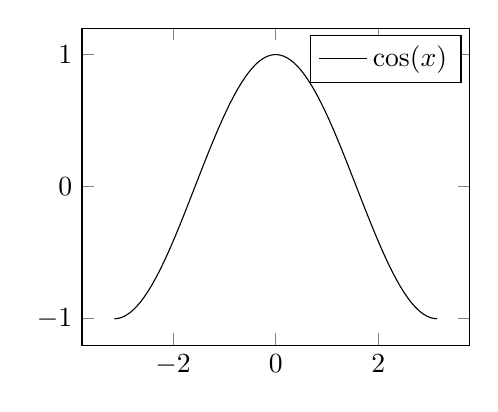
\begin{tikzpicture}
      \begin{axis}[width=6.5cm]
        \addplot [smooth,samples=100,domain=-pi:pi] {cos(deg(x))};
        \addlegendentry{$\cos(x)$};
      \end{axis}
    \end{tikzpicture}
    \caption*{PGFPlots}
  \end{subfigure}%
  \begin{subfigure}{0.5\linewidth}
    \centering
    \begin{tikzpicture}[gnuplot]
%% generated with GNUPLOT 5.4p1 (Lua 5.3; terminal rev. Jun 2020, script rev. 114)
%% 2021/07/04 17:20:13
\path (0.000,0.000) rectangle (6.500,5.000);
\gpcolor{color=gp lt color border}
\gpsetlinetype{gp lt border}
\gpsetdashtype{gp dt solid}
\gpsetlinewidth{1.00}
\draw[gp path] (1.196,0.616)--(1.376,0.616);
\draw[gp path] (5.947,0.616)--(5.767,0.616);
\node[gp node right] at (1.012,0.616) {$-1$};
\draw[gp path] (1.196,1.023)--(1.376,1.023);
\draw[gp path] (5.947,1.023)--(5.767,1.023);
\node[gp node right] at (1.012,1.023) {$-0.8$};
\draw[gp path] (1.196,1.431)--(1.376,1.431);
\draw[gp path] (5.947,1.431)--(5.767,1.431);
\node[gp node right] at (1.012,1.431) {$-0.6$};
\draw[gp path] (1.196,1.838)--(1.376,1.838);
\draw[gp path] (5.947,1.838)--(5.767,1.838);
\node[gp node right] at (1.012,1.838) {$-0.4$};
\draw[gp path] (1.196,2.246)--(1.376,2.246);
\draw[gp path] (5.947,2.246)--(5.767,2.246);
\node[gp node right] at (1.012,2.246) {$-0.2$};
\draw[gp path] (1.196,2.654)--(1.376,2.654);
\draw[gp path] (5.947,2.654)--(5.767,2.654);
\node[gp node right] at (1.012,2.654) {$0$};
\draw[gp path] (1.196,3.061)--(1.376,3.061);
\draw[gp path] (5.947,3.061)--(5.767,3.061);
\node[gp node right] at (1.012,3.061) {$0.2$};
\draw[gp path] (1.196,3.469)--(1.376,3.469);
\draw[gp path] (5.947,3.469)--(5.767,3.469);
\node[gp node right] at (1.012,3.469) {$0.4$};
\draw[gp path] (1.196,3.876)--(1.376,3.876);
\draw[gp path] (5.947,3.876)--(5.767,3.876);
\node[gp node right] at (1.012,3.876) {$0.6$};
\draw[gp path] (1.196,4.284)--(1.376,4.284);
\draw[gp path] (5.947,4.284)--(5.767,4.284);
\node[gp node right] at (1.012,4.284) {$0.8$};
\draw[gp path] (1.196,4.691)--(1.376,4.691);
\draw[gp path] (5.947,4.691)--(5.767,4.691);
\node[gp node right] at (1.012,4.691) {$1$};
\draw[gp path] (1.303,0.616)--(1.303,0.796);
\draw[gp path] (1.303,4.691)--(1.303,4.511);
\node[gp node center] at (1.303,0.308) {$-3$};
\draw[gp path] (2.059,0.616)--(2.059,0.796);
\draw[gp path] (2.059,4.691)--(2.059,4.511);
\node[gp node center] at (2.059,0.308) {$-2$};
\draw[gp path] (2.815,0.616)--(2.815,0.796);
\draw[gp path] (2.815,4.691)--(2.815,4.511);
\node[gp node center] at (2.815,0.308) {$-1$};
\draw[gp path] (3.572,0.616)--(3.572,0.796);
\draw[gp path] (3.572,4.691)--(3.572,4.511);
\node[gp node center] at (3.572,0.308) {$0$};
\draw[gp path] (4.328,0.616)--(4.328,0.796);
\draw[gp path] (4.328,4.691)--(4.328,4.511);
\node[gp node center] at (4.328,0.308) {$1$};
\draw[gp path] (5.084,0.616)--(5.084,0.796);
\draw[gp path] (5.084,4.691)--(5.084,4.511);
\node[gp node center] at (5.084,0.308) {$2$};
\draw[gp path] (5.840,0.616)--(5.840,0.796);
\draw[gp path] (5.840,4.691)--(5.840,4.511);
\node[gp node center] at (5.840,0.308) {$3$};
\draw[gp path] (1.196,4.691)--(1.196,0.616)--(5.947,0.616)--(5.947,4.691)--cycle;
\node[gp node right] at (4.479,4.357) {$\cos(x)$};
\gpcolor{rgb color={0.000,0.000,0.000}}
\draw[gp path] (4.663,4.357)--(5.579,4.357);
\draw[gp path] (1.196,0.616)--(1.244,0.620)--(1.292,0.632)--(1.340,0.653)--(1.388,0.681)%
  --(1.436,0.718)--(1.484,0.762)--(1.532,0.814)--(1.580,0.873)--(1.628,0.939)--(1.676,1.013)%
  --(1.724,1.093)--(1.772,1.179)--(1.820,1.271)--(1.868,1.369)--(1.916,1.472)--(1.964,1.579)%
  --(2.012,1.691)--(2.060,1.807)--(2.108,1.926)--(2.156,2.049)--(2.204,2.173)--(2.252,2.300)%
  --(2.300,2.428)--(2.348,2.557)--(2.396,2.686)--(2.444,2.815)--(2.492,2.943)--(2.540,3.071)%
  --(2.588,3.196)--(2.636,3.320)--(2.684,3.441)--(2.732,3.558)--(2.780,3.672)--(2.828,3.782)%
  --(2.876,3.887)--(2.924,3.988)--(2.972,4.083)--(3.020,4.172)--(3.068,4.255)--(3.116,4.332)%
  --(3.164,4.402)--(3.212,4.465)--(3.260,4.520)--(3.308,4.568)--(3.356,4.608)--(3.404,4.641)%
  --(3.452,4.665)--(3.500,4.682)--(3.548,4.690)--(3.595,4.690)--(3.643,4.682)--(3.691,4.665)%
  --(3.739,4.641)--(3.787,4.608)--(3.835,4.568)--(3.883,4.520)--(3.931,4.465)--(3.979,4.402)%
  --(4.027,4.332)--(4.075,4.255)--(4.123,4.172)--(4.171,4.083)--(4.219,3.988)--(4.267,3.887)%
  --(4.315,3.782)--(4.363,3.672)--(4.411,3.558)--(4.459,3.441)--(4.507,3.320)--(4.555,3.196)%
  --(4.603,3.071)--(4.651,2.943)--(4.699,2.815)--(4.747,2.686)--(4.795,2.557)--(4.843,2.428)%
  --(4.891,2.300)--(4.939,2.173)--(4.987,2.049)--(5.035,1.926)--(5.083,1.807)--(5.131,1.691)%
  --(5.179,1.579)--(5.227,1.472)--(5.275,1.369)--(5.323,1.271)--(5.371,1.179)--(5.419,1.093)%
  --(5.467,1.013)--(5.515,0.939)--(5.563,0.873)--(5.611,0.814)--(5.659,0.762)--(5.707,0.718)%
  --(5.755,0.681)--(5.803,0.653)--(5.851,0.632)--(5.899,0.620)--(5.947,0.616);
\gpcolor{color=gp lt color border}
\draw[gp path] (1.196,4.691)--(1.196,0.616)--(5.947,0.616)--(5.947,4.691)--cycle;
%% coordinates of the plot area
\gpdefrectangularnode{gp plot 1}{\pgfpoint{1.196cm}{0.616cm}}{\pgfpoint{5.947cm}{4.691cm}}
\end{tikzpicture}
%% gnuplot variables

    \caption*{gnuplot-lua-tikz}
  \end{subfigure}

  \bigskip
  \begin{subfigure}{0.5\linewidth}
    \centering
    \begin{tikzpicture}
      \begin{axis}[width=6.5cm]
        \addplot [smooth,samples=100,mark=none,domain=-pi:pi] function [id=cos] {cos(x)};
        \addlegendentry{$\cos(x)$};
      \end{axis}
    \end{tikzpicture}
    \caption*{GNUPlot on PGFPlots}
  \end{subfigure}%
  \begin{subfigure}{0.5\linewidth}
    \centering
    \begin{tikzpicture}
      \datavisualization [
        scientific axes,
        visualize as smooth line/.list={cosine},
        x axis={length=4.5cm},
        y axis={length=4cm},
        legend=north east inside,
        cosine={label in legend={text={$\cos(x)$}}}]
      data [set=cosine, format=function] {
        var x : interval [-pi:pi] samples 100;
        func y = cos(deg(\value x));
      };
    \end{tikzpicture}
    \caption*{datavisualization}
  \end{subfigure}
  \caption{グラフ描画の比較}
\end{figure}

\begin{codeblock}
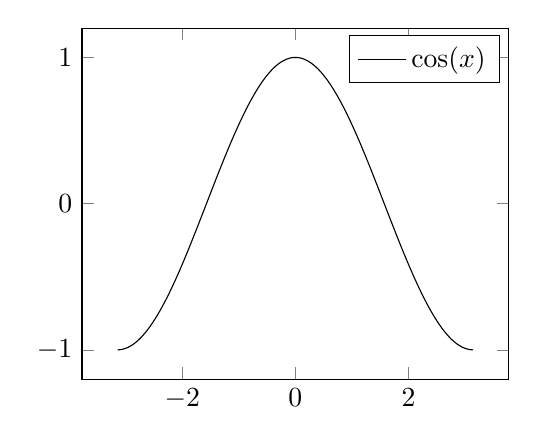
\begin{tikzpicture}
  \begin{axis}[width=7cm]
    \addplot [smooth,samples=100,domain=-pi:pi] {cos(deg(x))};
    \addlegendentry{$\cos(x)$};
  \end{axis}
\end{tikzpicture}
\end{codeblock}

\begin{codeblock}
\begin{tikzpicture}[gnuplot]
%% generated with GNUPLOT 5.4p1 (Lua 5.3; terminal rev. Jun 2020, script rev. 114)
%% 2021/07/04 17:20:13
\path (0.000,0.000) rectangle (6.500,5.000);
\gpcolor{color=gp lt color border}
\gpsetlinetype{gp lt border}
\gpsetdashtype{gp dt solid}
\gpsetlinewidth{1.00}
\draw[gp path] (1.196,0.616)--(1.376,0.616);
\draw[gp path] (5.947,0.616)--(5.767,0.616);
\node[gp node right] at (1.012,0.616) {$-1$};
\draw[gp path] (1.196,1.023)--(1.376,1.023);
\draw[gp path] (5.947,1.023)--(5.767,1.023);
\node[gp node right] at (1.012,1.023) {$-0.8$};
\draw[gp path] (1.196,1.431)--(1.376,1.431);
\draw[gp path] (5.947,1.431)--(5.767,1.431);
\node[gp node right] at (1.012,1.431) {$-0.6$};
\draw[gp path] (1.196,1.838)--(1.376,1.838);
\draw[gp path] (5.947,1.838)--(5.767,1.838);
\node[gp node right] at (1.012,1.838) {$-0.4$};
\draw[gp path] (1.196,2.246)--(1.376,2.246);
\draw[gp path] (5.947,2.246)--(5.767,2.246);
\node[gp node right] at (1.012,2.246) {$-0.2$};
\draw[gp path] (1.196,2.654)--(1.376,2.654);
\draw[gp path] (5.947,2.654)--(5.767,2.654);
\node[gp node right] at (1.012,2.654) {$0$};
\draw[gp path] (1.196,3.061)--(1.376,3.061);
\draw[gp path] (5.947,3.061)--(5.767,3.061);
\node[gp node right] at (1.012,3.061) {$0.2$};
\draw[gp path] (1.196,3.469)--(1.376,3.469);
\draw[gp path] (5.947,3.469)--(5.767,3.469);
\node[gp node right] at (1.012,3.469) {$0.4$};
\draw[gp path] (1.196,3.876)--(1.376,3.876);
\draw[gp path] (5.947,3.876)--(5.767,3.876);
\node[gp node right] at (1.012,3.876) {$0.6$};
\draw[gp path] (1.196,4.284)--(1.376,4.284);
\draw[gp path] (5.947,4.284)--(5.767,4.284);
\node[gp node right] at (1.012,4.284) {$0.8$};
\draw[gp path] (1.196,4.691)--(1.376,4.691);
\draw[gp path] (5.947,4.691)--(5.767,4.691);
\node[gp node right] at (1.012,4.691) {$1$};
\draw[gp path] (1.303,0.616)--(1.303,0.796);
\draw[gp path] (1.303,4.691)--(1.303,4.511);
\node[gp node center] at (1.303,0.308) {$-3$};
\draw[gp path] (2.059,0.616)--(2.059,0.796);
\draw[gp path] (2.059,4.691)--(2.059,4.511);
\node[gp node center] at (2.059,0.308) {$-2$};
\draw[gp path] (2.815,0.616)--(2.815,0.796);
\draw[gp path] (2.815,4.691)--(2.815,4.511);
\node[gp node center] at (2.815,0.308) {$-1$};
\draw[gp path] (3.572,0.616)--(3.572,0.796);
\draw[gp path] (3.572,4.691)--(3.572,4.511);
\node[gp node center] at (3.572,0.308) {$0$};
\draw[gp path] (4.328,0.616)--(4.328,0.796);
\draw[gp path] (4.328,4.691)--(4.328,4.511);
\node[gp node center] at (4.328,0.308) {$1$};
\draw[gp path] (5.084,0.616)--(5.084,0.796);
\draw[gp path] (5.084,4.691)--(5.084,4.511);
\node[gp node center] at (5.084,0.308) {$2$};
\draw[gp path] (5.840,0.616)--(5.840,0.796);
\draw[gp path] (5.840,4.691)--(5.840,4.511);
\node[gp node center] at (5.840,0.308) {$3$};
\draw[gp path] (1.196,4.691)--(1.196,0.616)--(5.947,0.616)--(5.947,4.691)--cycle;
\node[gp node right] at (4.479,4.357) {$\cos(x)$};
\gpcolor{rgb color={0.000,0.000,0.000}}
\draw[gp path] (4.663,4.357)--(5.579,4.357);
\draw[gp path] (1.196,0.616)--(1.244,0.620)--(1.292,0.632)--(1.340,0.653)--(1.388,0.681)%
  --(1.436,0.718)--(1.484,0.762)--(1.532,0.814)--(1.580,0.873)--(1.628,0.939)--(1.676,1.013)%
  --(1.724,1.093)--(1.772,1.179)--(1.820,1.271)--(1.868,1.369)--(1.916,1.472)--(1.964,1.579)%
  --(2.012,1.691)--(2.060,1.807)--(2.108,1.926)--(2.156,2.049)--(2.204,2.173)--(2.252,2.300)%
  --(2.300,2.428)--(2.348,2.557)--(2.396,2.686)--(2.444,2.815)--(2.492,2.943)--(2.540,3.071)%
  --(2.588,3.196)--(2.636,3.320)--(2.684,3.441)--(2.732,3.558)--(2.780,3.672)--(2.828,3.782)%
  --(2.876,3.887)--(2.924,3.988)--(2.972,4.083)--(3.020,4.172)--(3.068,4.255)--(3.116,4.332)%
  --(3.164,4.402)--(3.212,4.465)--(3.260,4.520)--(3.308,4.568)--(3.356,4.608)--(3.404,4.641)%
  --(3.452,4.665)--(3.500,4.682)--(3.548,4.690)--(3.595,4.690)--(3.643,4.682)--(3.691,4.665)%
  --(3.739,4.641)--(3.787,4.608)--(3.835,4.568)--(3.883,4.520)--(3.931,4.465)--(3.979,4.402)%
  --(4.027,4.332)--(4.075,4.255)--(4.123,4.172)--(4.171,4.083)--(4.219,3.988)--(4.267,3.887)%
  --(4.315,3.782)--(4.363,3.672)--(4.411,3.558)--(4.459,3.441)--(4.507,3.320)--(4.555,3.196)%
  --(4.603,3.071)--(4.651,2.943)--(4.699,2.815)--(4.747,2.686)--(4.795,2.557)--(4.843,2.428)%
  --(4.891,2.300)--(4.939,2.173)--(4.987,2.049)--(5.035,1.926)--(5.083,1.807)--(5.131,1.691)%
  --(5.179,1.579)--(5.227,1.472)--(5.275,1.369)--(5.323,1.271)--(5.371,1.179)--(5.419,1.093)%
  --(5.467,1.013)--(5.515,0.939)--(5.563,0.873)--(5.611,0.814)--(5.659,0.762)--(5.707,0.718)%
  --(5.755,0.681)--(5.803,0.653)--(5.851,0.632)--(5.899,0.620)--(5.947,0.616);
\gpcolor{color=gp lt color border}
\draw[gp path] (1.196,4.691)--(1.196,0.616)--(5.947,0.616)--(5.947,4.691)--cycle;
%% coordinates of the plot area
\gpdefrectangularnode{gp plot 1}{\pgfpoint{1.196cm}{0.616cm}}{\pgfpoint{5.947cm}{4.691cm}}
\end{tikzpicture}
%% gnuplot variables

\end{codeblock}

\begin{codeblock}
gnuplot> set terminal lua tikz size 7cm,5cm
gnuplot> set output "gnuplot.tex"
gnuplot> set xrange [-pi:pi]
gnuplot> plot cos(x) linetype rgb "black" title '$\cos(x)$'
gnuplot> exit
\end{codeblock}

\begin{codeblock}
\begin{tikzpicture}
  \begin{axis}[width=7cm]
    \addplot [smooth,samples=100,mark=none,domain=-pi:pi] function [id=cos] {cos(x)};
    \addlegendentry{$\cos(x)$};
  \end{axis}
\end{tikzpicture}
\end{codeblock}

\begin{codeblock}
\begin{tikzpicture}
  \datavisualization [
    scientific axes,
    visualize as smooth line/.list={cosine},
    x axis={length=5cm},
    y axis={length=4cm},
    legend=north east inside,
    cosine={label in legend={text={$\cos(x)$}}}]
  data [set=cosine, format=function] {
    var x : interval [-pi:pi] samples 100;
    func y = cos(deg(\value x));
  };
\end{tikzpicture}
\end{codeblock}

\section{その他のグラフ}
3Dグラフなども同様の要領で作成できる.以下にPGFPlotsを利用した例を示す.

\begin{codeblock}
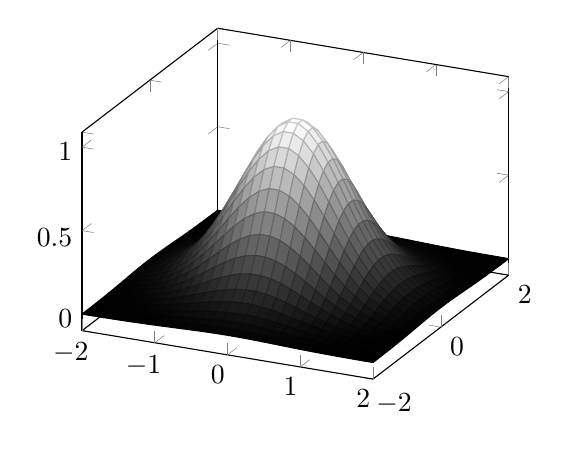
\begin{tikzpicture}
  \begin{axis}[width=7cm,colormap/blackwhite]
    \addplot3 [surf,miter limit=1,samples=30,domain=-2:2] {exp(-(x^2+y^2))};
  \end{axis}
\end{tikzpicture}
\end{codeblock}

\begin{figure}[ht]
  \centering
  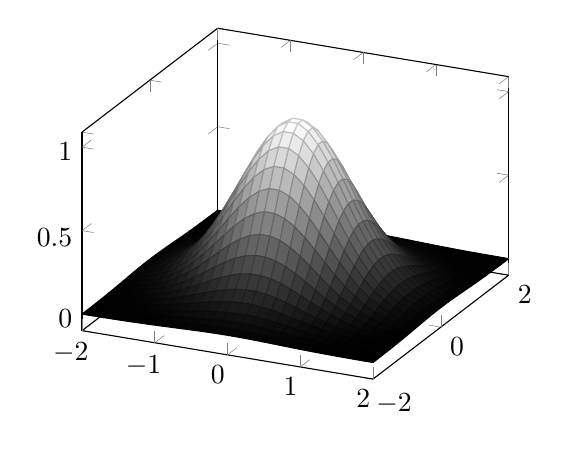
\begin{tikzpicture}
    \begin{axis}[width=7cm,colormap/blackwhite]
      \addplot3 [surf,miter limit=1,samples=30,domain=-2:2] {exp(-(x^2+y^2))};
    \end{axis}
  \end{tikzpicture}
  \caption{$e^{-(x^2+y^2)}$のグラフ}
\end{figure}

\section{補遺}
\subsection{グラフ描画の精度}
PGFPlotsのRevision 1.18 (2021/05/08) p.54を引用する.

\begin{quotation}
  \textbf{About the precision and number range:} Starting with version 1.2, \inlinecode{\addplot expression} uses
  a floating point unit. The FPU provides the full data range of scientific computing with a relative
  precision between $10^{-4}$ and $10^{-6}$. The \inlinecode{/pgf/fpu} key provides some more details.

  Note that pgfplots makes use of lualatex's features: if you use lualatex instead of pdflatex,
  pgfplots will use lua's math engine which is both faster and more accurate (\inlinecode{compat=1.12} or higher).
\end{quotation}

つまり,処理系が\LuaLaTeX であり,\inlinecode{compat}に1.12以上のバージョンが指定されていれば,
PGFPlotsはLuaの数学エンジンを利用して計算を行う.これは\TeX 上の実装より高速かつ正確である.
\end{document}
